\documentclass[border=10pt]{standalone}
\usepackage{tikz}\usepackage{amsmath}\usetikzlibrary{arrows.meta}
\begin{document}
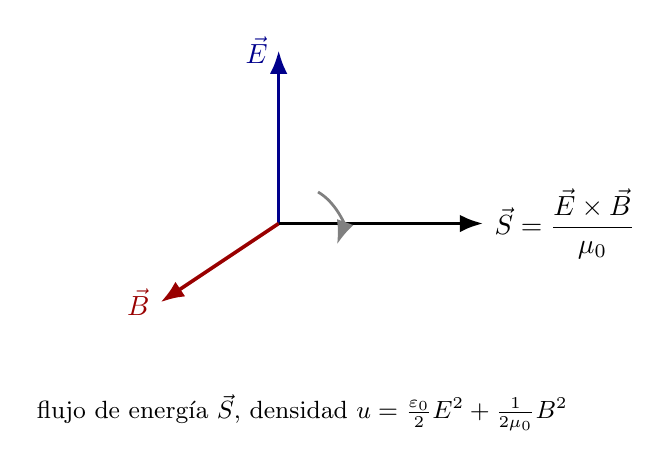
\begin{tikzpicture}[line width=1pt,>={Latex[length=3mm]}]
  \coordinate (O) at (0,0);
  \draw[->,blue!55!black,line width=1.3pt] (O)--(0,2.2) node[left]{$\vec E$};
  \draw[->,red!60!black,line width=1.3pt] (O)--(-1.5,-1.0) node[left]{$\vec B$};
  \draw[->,black,line width=1.4pt] (O)--(2.6,0) node[right]{$\vec S=\dfrac{\vec E\times\vec B}{\mu_0}$};
  \draw[->,gray] (0.5,0.4) arc (60:-20:0.55);
  \node at (0.3,-2.4){\small flujo de energía $\vec S$, densidad $u=\tfrac{\varepsilon_0}{2}E^2+\tfrac{1}{2\mu_0}B^2$};
\end{tikzpicture}
\end{document}
